\chapter{The analysis, validated before the data}
\label{ch:participant}

\noindent
\fbox{\parbox{0.955\linewidth}{\centering\bfseries
No participant data has been collected.\\[4pt]
\normalfont\small
The study of \cref{ch:study} has not been run. This chapter therefore
reports what \emph{can} be established without participants, which is more
than nothing and less than a result: the analysis that will be applied,
written out in full, and a measurement of how that analysis behaves on data
whose answer is known. The reason no session has been run is not
administrative and is stated in \cref{sec:blocked}.}}

\bigskip

An analysis specified but never executed is an assumption. The pre-registered
plan for this study carries one number --- \SI{80}{\percent} power to detect
$d = \num{0.73}$ at sixteen dyads --- and that number came from a power
formula for a single paired comparison, while the analysis that will actually
be run applies a family-wise correction across five of them. Those are
different quantities, and the difference is not small. This chapter measures
it.

\section{The analysis, written out}
\label{sec:analysis-spec}

The design is within dyads: every dyad performs every condition, so the unit
of analysis is the paired difference and not the raw score. For task $j$, with
$y^{\text{DT}}_{ij}$ and $y^{\text{SA}}_{ij}$ the outcome for dyad $i$ under
direct teleoperation and shared autonomy,

\begin{equation}
  \label{eq:paired-diff}
  d_{ij} = y^{\text{SA}}_{ij} - y^{\text{DT}}_{ij},
  \qquad
  t_j = \frac{\bar{d}_{\cdot j}}{s_{d,j}/\sqrt{n}},
  \qquad
  \nu = n - 1 .
\end{equation}

The effect size reported alongside is the standardised mean of those
differences, which is the quantity the design was powered for and is not the
same as the standardised difference of the two means:

\begin{equation}
  \label{eq:dz}
  d_z = \frac{\bar{d}_{\cdot j}}{s_{d,j}} .
\end{equation}

The distinction is worth stating because conflating the two deflates every
effect by a factor of $\sqrt{2}$ when the two conditions are uncorrelated, and
by more when they are positively correlated, which within a dyad they are.

Five tasks give a family of five comparisons. The pre-registered correction is
Holm's step-down procedure: with the raw values sorted ascending as
$p_{(1)} \le \dots \le p_{(m)}$,

\begin{equation}
  \label{eq:holm}
  \tilde{p}_{(k)} = \max_{l \le k}\;
    \min\bigl\{(m - l + 1)\,p_{(l)},\; 1\bigr\} ,
\end{equation}

the outer maximum enforcing monotonicity so that a comparison cannot be
declared significant while a stronger one is not. Holm controls the family-wise
error rate at $\alpha$ under any dependence structure and is uniformly more
powerful than the plain Bonferroni bound it refines, so there is no
configuration in which Bonferroni would be preferred.

\section{What the analysis does to data whose answer is known}
\label{sec:pipeline-validation}

\Cref{eq:paired-diff,eq:dz,eq:holm} were applied to constructed data:
\num{20000} simulated studies at the planned sixteen dyads, each with five
contrasts, in two conditions. In the first, a true effect of exactly
$d_z = \num{0.73}$ was added to every contrast. In the second, no effect was
added at all. Both were pushed through the same implementation the study will
use --- \repo{srl\_experiments/posthoc.py}, unmodified --- by
\repo{scripts/validate\_analysis\_pipeline.py}.

This is the one place in this thesis where synthetic data is admissible, and
it is admissible for a specific reason: the ground truth is \emph{constructed}
--- a constant added to a sample --- rather than \emph{rendered}. Nothing here
is a claim about the platform. It is a measurement of the analysis.

\begin{table}[htbp]
  \centering
  \caption[The analysis on constructed data]{The pre-registered analysis
  applied to \num{20000} simulated studies per row at $n = 16$ dyads,
  $m = 5$ contrasts, $\alpha = \num{0.05}$. The null row is the check that
  can fail: a procedure that rejects everything has perfect power and is
  worthless, so the false-positive rate is reported beside the power and must
  come out at $\alpha$. It does, to three decimal places, which is what
  licenses reading the row above it.}
  \label{tab:pipeline-validation}
  \begin{tabular}{@{}lccc@{}}
    \toprule
    & \multicolumn{3}{c}{probability of rejecting $H_0$} \\
    \cmidrule(l){2-4}
    Constructed truth & one contrast, & one contrast, & some contrast \\
                      & uncorrected   & Holm-corrected & in the family \\
    \midrule
    $d_z = \num{0.73}$ on all five & \num{0.777} & \num{0.638} & \num{0.973} \\
    no effect at all               & \num{0.052} & \num{0.010} & \num{0.050} \\
    \bottomrule
  \end{tabular}
\end{table}

\begin{figure}[htbp]
  \centering
  % POWER AGAINST THE NUMBER OF DYADS, from
% scripts/validate_analysis_pipeline.py, 6000 simulated studies per point.
% Three curves because the design carries ONE number and the analysis that
% will be run reports three different things.
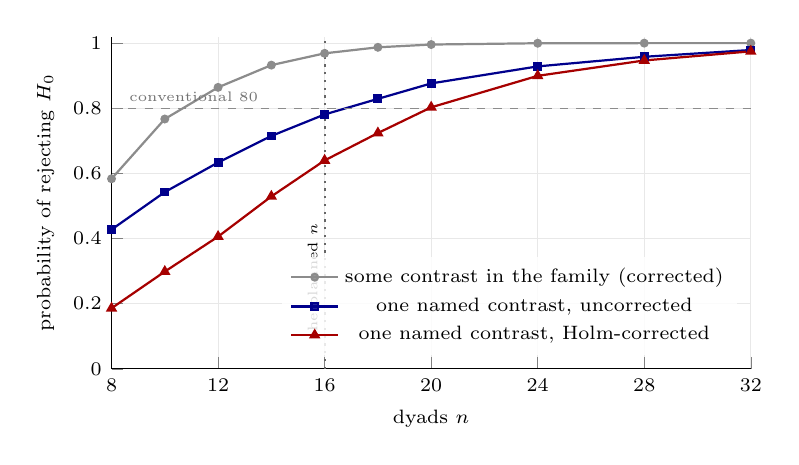
\begin{tikzpicture}
\begin{axis}[
    width=0.80\linewidth, height=58mm,
    xmin=8, xmax=32, ymin=0, ymax=1.02,
    xlabel={dyads $n$}, ylabel={probability of rejecting $H_0$},
    xlabel style={font=\scriptsize}, ylabel style={font=\scriptsize},
    tick label style={font=\scriptsize},
    legend style={font=\scriptsize, at={(0.98,0.04)}, anchor=south east,
                  draw=none, fill=white, fill opacity=0.85, text opacity=1},
    axis lines*=left, grid=major, grid style={gray!18},
    xtick={8,12,16,20,24,28,32},
]
\addplot[black!45, thick, mark=*, mark size=1.2pt] coordinates {
  (8,0.5835) (10,0.7670) (12,0.8642) (14,0.9325) (16,0.9687)
  (18,0.9872) (20,0.9957) (24,0.9997) (28,1.0000) (32,1.0000)};
\addlegendentry{some contrast in the family (corrected)}
\addplot[blue!55!black, thick, mark=square*, mark size=1.2pt] coordinates {
  (8,0.4275) (10,0.5427) (12,0.6335) (14,0.7150) (16,0.7810)
  (18,0.8289) (20,0.8763) (24,0.9286) (28,0.9581) (32,0.9789)};
\addlegendentry{one named contrast, uncorrected}
\addplot[red!65!black, thick, mark=triangle*, mark size=1.6pt] coordinates {
  (8,0.1859) (10,0.2985) (12,0.4059) (14,0.5293) (16,0.6398)
  (18,0.7239) (20,0.8029) (24,0.8996) (28,0.9468) (32,0.9748)};
\addlegendentry{one named contrast, Holm-corrected}
\draw[black!45, dashed] (axis cs:8,0.8) -- (axis cs:32,0.8);
\node[font=\tiny, black!55, anchor=west] at (axis cs:8.3,0.835) {conventional \SI{80}{\percent}};
\draw[black!60, dotted, thick] (axis cs:16,0) -- (axis cs:16,1.02);
\node[font=\tiny, anchor=south west, rotate=90] at (axis cs:16.2,0.06) {the planned $n$};
\end{axis}
\end{tikzpicture}

  \caption[Power against the number of dyads]{Power against the number of
  dyads at $d_z = \num{0.73}$, from \num{6000} simulated studies per point.
  The design's stated \SI{80}{\percent} is the middle curve read at
  $n = \num{16}$, and it is met. The lower curve is the same contrast after
  the correction the analysis actually applies, and the upper curve is the
  probability that \emph{some} contrast in the family survives. The three
  answer three different questions and the design records only the middle
  one.}
  \label{fig:power}
\end{figure}

Three things follow, and none of them was in the design.

\textbf{The design's own number is confirmed, and it is the wrong number to
plan with.} An uncorrected paired contrast at sixteen dyads recovers a
$d_z = \num{0.73}$ effect \SI{77.7}{\percent} of the time, which reproduces
the planning calculation. But no contrast will be reported uncorrected,
because there are five of them.

\textbf{The correction costs fourteen percentage points.} After Holm, the
probability of recovering the effect on a \emph{named} task falls to
\SI{63.8}{\percent}. \Cref{fig:power} shows that restoring
\SI{80}{\percent} on a named task needs twenty dyads rather than sixteen ---
eight additional participants, or roughly two additional laboratory days at
the session length of \cref{fig:timeline}.

\textbf{The study is nevertheless well powered for the claim it is making.}
The probability that at least one contrast in the family survives correction
is \SI{97.3}{\percent}. The design's question is whether shared autonomy
changes performance on this platform, not whether it changes performance on
task T3 specifically, and for that question sixteen dyads is ample. The
consequence for reporting is precise: a per-task null result at $n = 16$ is
not evidence of no per-task effect, and must be reported as an interval rather
than as an absence.

The null row of \cref{tab:pipeline-validation} is the half of this measurement
that could have failed. A family-wise false-positive rate of \num{0.050}
against a nominal $\alpha = \num{0.05}$ establishes that the correction is
implemented as specified rather than merely called; the per-contrast rate of
\num{0.010} is the $\alpha/m$ the step-down procedure is expected to leave at
the first step.

\section{What the session will report}
\label{sec:reporting-plan}

The outputs below are fixed in advance so that the choice of what to report
cannot be made after seeing the data. Each names the quantity, the test, and
the reason the decomposition is what it is; none is drawn here, because a
figure of no data is not a figure.

\begin{table}[htbp]
  \centering
  \small
  \caption[The reporting plan]{Every output the session produces, fixed
  before data collection. Where a measure is reported separately by role,
  the reason is that the two roles load differently and pooling them would
  average away the contrast the two-person design exists to expose: only the
  wearer carries \SI{17}{\kilo\gram}, and only the operator holds an
  uncompensated master arm against gravity.}
  \label{tab:reporting-plan}
  \begin{tabular}{@{}p{0.24\linewidth}p{0.30\linewidth}p{0.38\linewidth}@{}}
    \toprule
    Quantity & Test & Decomposition, and why \\
    \midrule
    Completion time
      & paired contrast per task, Holm across five
      & per task; T2 has no mode contrast (\cref{sec:cells}) and is reported
        as a single condition \\
    Coordination error
      & threshold crossing rate, T3 and T4
      & against the measured failure thresholds, \SI{6.8}{\degree} of tray
        tilt and \SI{534}{\milli\metre} of gripper separation \\
    Cross-arm interference
      & regression of one arm's tracking error on the other arm's target
        speed, T5
      & the slope reported beside the phase lag: a large slope with a flat
        lag is attentional, both rising together is not \\
    Grasp success
      & proportion, autonomy conditions only
      & no teleoperation row exists and none should be added
        (\cref{sec:cells}) \\
    NASA-TLX~\cite{hart1988nasatlx}
      & six subscales and the weighted total
      & operator and wearer separately \\
    Borg CR10~\cite{borg1982perceived}
      & slope across blocks, not endpoint
      & fatigue is monotonic in time, so the slope is the quantity and the
        endpoint is a confound \\
    Trust
      & by autonomy level, wearer only
      & against the prediction that higher autonomy \emph{lowers} wearer
        trust~\cite{zhou2026proxemics} \\
    Embodiment
      & ownership, agency and location separately
      & the components move independently~\cite{longo2008embodiment} and a
        single score hides that \\
    Proprioceptive drift
      & paired, pre against post
      & reported per participant against the unity line; two means discard
        the pairing the design bought \\
    \bottomrule
  \end{tabular}
\end{table}

Two constraints on reporting follow from \cref{sec:pipeline-validation} and
are stated here rather than discovered later. Effects are reported as
estimates with intervals whether or not they cross the threshold, because at
$n = 16$ a per-task null is uninformative on its own. And the exchange rate
between operator performance and wearer trust --- the quantity the two-person
framing makes interesting --- is a correlation \emph{across} roles, which this
design was not powered for; it is reported descriptively with an interval and
no test.

\section{Safety events}

\begin{table}[htbp]
  \centering
  \small
  \caption[Safety events during sessions]{Everything the safety layer does
  during a session, recorded automatically rather than by an observer. This
  table is reported whether or not anything happens: a table of zeros is a
  result, and its absence is indistinguishable from a table that was never
  produced. No field in it identifies a participant;
  \repo{write\_manifest()} raises on name, electronic mail address, date of
  birth, address and telephone number, so anonymity is enforced by the code
  that writes the record rather than by the person writing it up.}
  \label{tab:safety-events}
  \begin{tabular}{@{}lcc@{}}
    \toprule
    Event & Direct teleoperation & Shared autonomy \\
    \midrule
    Emergency stops, and by whom & --- & --- \\
    Clearance holds & --- & --- \\
    Minimum recorded clearance & --- & --- \\
    Trials invalidated by a fault, with cause & --- & --- \\
    Sessions ended at a participant's request & --- & --- \\
    \bottomrule
  \end{tabular}
\end{table}

\section{Why no session has been run}
\label{sec:blocked}

Two independent blocks, neither of which is a matter of scheduling.

The first is technical and is measured in \cref{ch:results}: the direct
teleoperation condition is the baseline of every comparison in
\cref{tab:reporting-plan}, and it depends on master channels of which six of
fourteen currently meet the coherence criterion. The failing channels are a
soldering problem at two identified joints, and until they are repaired the
baseline condition would be measuring the master arm's wiring rather than the
operator.

The second is ethical and is not resolved by repairing anything. The wearer
and the operator are different people who consent separately, and worn
operation places more than \SI{17}{\kilo\gram} on someone who is not
commanding the motion and has no gravity compensation. \Cref{ch:discussion}
sets out, in priority order, what stands between the system as built and a
session with two people in it. The first item on that list is two soldered
joints; the second is an approved protocol.
